\section{On text, extra loops at inference never help}
\label{sec:mechanism}

If the loop iterated towards an answer, the state after each loop would carry a better prediction than the state
before it, and running more loops at inference would help. At these sizes, it does not. To see what the loop computes
instead, we probed trained models loop by loop, on trunk checkpoints at $32N$ before cooldown \lbl{(exploratory)}. We
read the state after each loop with the model's own output layers (the coda and the output head), with a learned
linear map placed before them, and with a learned linear head in their place (Appendix~\ref{app:fits}). Reading it
through the model's own output layers, a logit lens, is the same as running the model with that many loops; the learned
map is a tuned lens trained on the next token. Figure~\ref{fig:mechanism} shows three training regimes.

\begin{figure}[t]
  \centering
  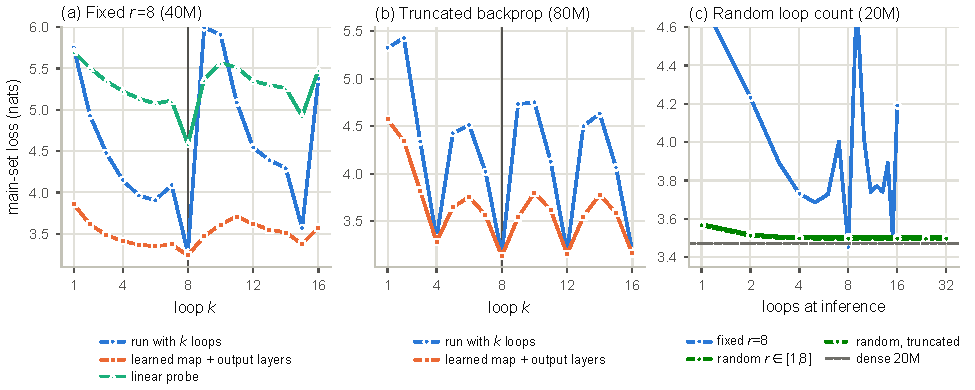
\includegraphics[width=\linewidth]{fig4_text_mechanism}
  \caption{What the looped block computes on text (main-set loss of trunk checkpoints at $32N$; values above the top of
  a panel are clipped). \textbf{(a)}~Fixed loop count: a 40M middle block trained with 8 loops (mean of three seeds),
  read after each loop $k$ by running the model with $k$ loops, by a learned linear map placed before the output layers,
  and by a learned linear head in their place. The model reaches its low loss only at its training loop count. \textbf{(b)}~Truncated backpropagation (80M
  whole stack, $r = 8$, gradients through the last 4 loops): the state returns to almost the same point every four loops.
  \textbf{(c)}~Trained with a random loop count (20M middle block, $r$ drawn from 1--8 at every training step), the block
  contracts to a fixed point: the loss is flat from about four loops on and no better than the dense model, with or
  without truncation.}
  \label{fig:mechanism}
\end{figure}

Trained with a fixed count of 8 loops, the middle block behaves like a fixed-length program. The model reaches its low
loss only at 8 loops, and running it with fewer or more loops makes the loss much higher (Figure~\ref{fig:mechanism}a).
Read with a learned map, the state after loop 4 is already within 0.1--0.2 nats of the final loss, and loops 5--7 add
little. The last loop is a large non-linear move that rewrites the state into what the output layers expect: for
37--47\% of the tokens, the predicted token changes for the last time at loop 8. These patterns held in all three seeds
at 20M and 40M, and in the one seed at 80M.

With truncated backpropagation, the whole stack learns a periodic cycle. When it is trained with 8 loops and gradients
through only the last four, its state returns to almost the same point every four loops (Figure~\ref{fig:mechanism}b).
The model works at 4, 8, 12 or 16 loops and gains nothing from more loops. The same minima at 4, 8 and 12
loops appear at 20M and in both probed 40M seeds. We did not probe a middle block trained with truncated backpropagation.

Drawing the loop count from 1--8 at every training step, as Huginn does with a different distribution
\citep{geiping2025scaling}, gives a block that contracts to a fixed point. Its loss is flat from about four loops to 32
(Figure~\ref{fig:mechanism}c; one seed at 20M, with full and with truncated backpropagation). Such a model is robust to
the loop count, but at 8 loops, the top of its training range, it is 0.05 nats worse than the model trained with a
fixed 8 loops and no better than the dense model. Parcae's models, trained with a sampled loop count at 140M--770M, keep
an advantage, so our result, from one seed at one size, may be specific to small models or to our distribution.

Lower learning rates give flatter curves over the inference loop count. In S1, whose plan lists this as an exploratory
question (Q5), the loss of the 4-loop model at 10M, 20M and 40M varies by 0.36--0.77 nats over 4--16 loops at 0.5 times
the dense rate, and by 3.4--4.6 nats at 1.41 times. At every rate, though, the better of 8 and 16 loops was worse than
the training count of 4.

The looped model's gain over the dense model on web text is small and spread across tokens \lbl{(exploratory)}. About
half of the tokens improve, and the gain is no more concentrated on hard tokens than the difference between two dense
seeds is. On math and code text the gains are larger, but there the spread between seeds is 10--100 times larger as
well, and the code set is more sensitive to the data order than to the initialisation (S7, \lbl{pre-specified};
Appendix~\ref{app:fits}). We draw no conclusions from differences on those sets.

On web text at these sizes, then, the loop gains little from iterating, and running it for more loops than it was
trained with never helped.
